\hypertarget{problem-summary}{%
\section{Problem Summary}\label{problem-summary}}

I worked on implementing the Marching Cubes algorithm for my final
project. Marching Cubes is an isosurface extraction algorithm that is
quite popular and has spurned quite a lot of research in the computer
graphics community. It has a certain elegance and simplicity to it and
is also quite fast in nature when compared to direct rendering based
methods. It is important from the point of view of vizualization
applications involving 3D data.

\hypertarget{description-of-work}{%
\section{Description of Work}\label{description-of-work}}

\begin{itemize}
\tightlist
\item
  Algorithm description -- hand drawing of marching squares
\item
  Reading about the alogorithm and its implementation aspects -- filling
  the grid points with values interpolated from the raw data voxels.
\item
  Using the lookup tables to obtain interpolated vertices on edges of a
  single cell and forming a triangular face.
\item
  Constructing a normal for the face by taking a cross product between
  the difference of two vertices -- making a custom struct to hold the
  vertex position and normal vectors.
\item
  Finally integrating it into the existing pipeline of: Camera,
  Lighting, Object, and Renderer classes in the code. Using the normal
  information, I could use the basic Phong model to show the scene.
\item
  Also downloaded additional 3D raw data files from internet
  (https://klacansky.com/open-scivis-datasets/) to showcase the results.
\end{itemize}

\hypertarget{challenges}{%
\subsection{Challenges}\label{challenges}}

\begin{itemize}
\tightlist
\item
  indexing into the grid and voxel data depending on the number of cuts.
  Was a bit non-intuitive at first and need careful attention to avoid
  mistakes in indexing!
\item
  can try to have a better normal representation for each vertex:
  probably by taking the average of normals across all the faces that
  the vertex lies on.
\end{itemize}

\hypertarget{results}{%
\section{Results}\label{results}}

A complete C++/OpenGL GUI application has been developed as a part of
the project. The GUI allows to change the following variables related to
marching cubes algorithm:

\begin{itemize}
\tightlist
\item
  3D volume data set
\item
  Number of slices (Grid resolution, higher is better)
\item
  Isovalue: Value at which to extract the surface
\end{itemize}

In addition GUI knobs for parameters like rendering type, camera
movement, lighting etc are also provided for ease of use. Figures are
included with appropriate captions in order to demonstrate some
rendering results across different data sets.

\begin{figure}
\centering
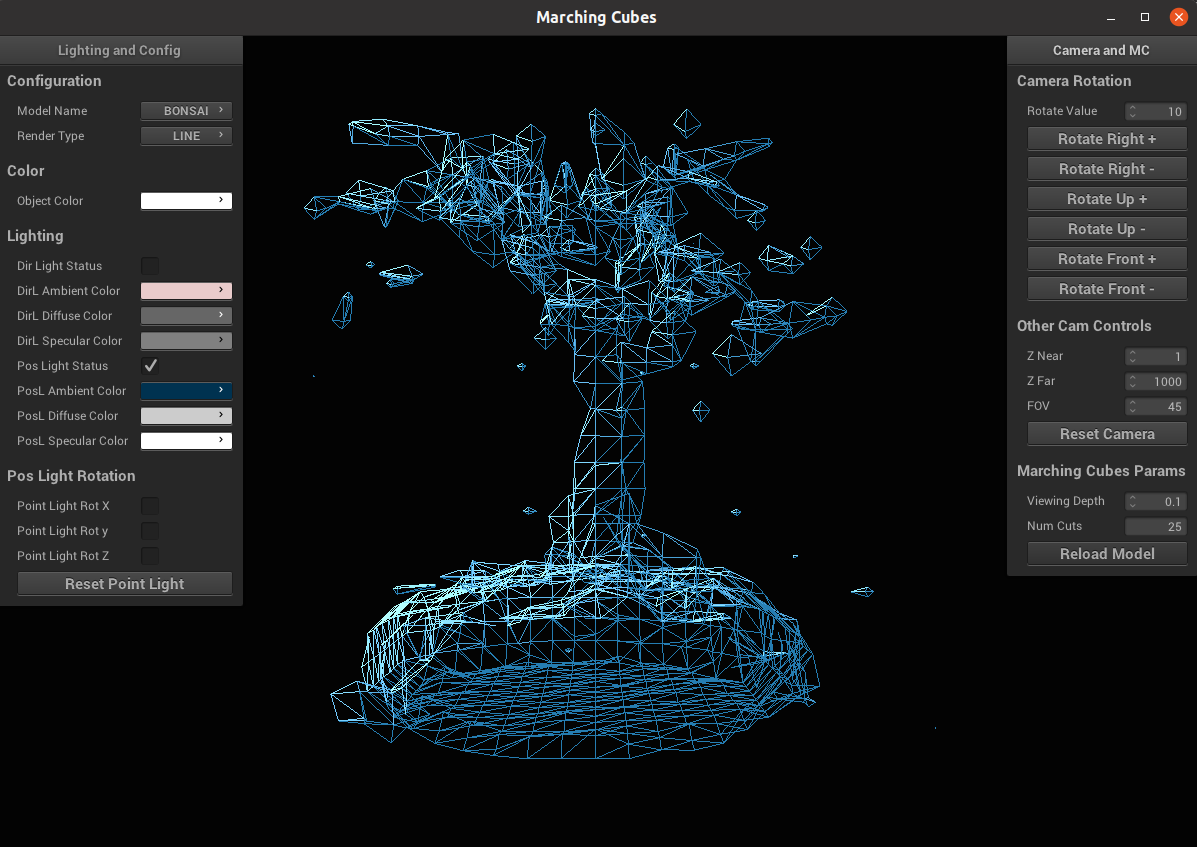
\includegraphics{./screenshots/meshing/bonsai_mesh.png}
\caption{Bonsai Mesh}
\end{figure}

\hypertarget{analysis-of-work}{%
\section{Analysis of Work}\label{analysis-of-work}}

I believe that I was successful in my main aim of understanding and
implementing marching cubes algorithm. I had taken up this project (and
changed my original proposal) in order to learn something different and
give myself know how about a technique which is widely used. However I
can see an area of improvement in terms of better shading techniques for
the 3d models. This needs more accuract normal computation for the
vertex data points which I was not able to finish due to a lack of time
but I will try to take this up later on as I suspect (and hope!) that I
might not need to change my code too much. Apart from the above point, I
plan to continue reading about extensions to the original algorithm and
related techniques like dual contouring etc. as I have gained the
prerequisite knowledge to go through the different techniques. I had
initially thought about implementing dual contouring as well but could
not do this since I based my code heavily on the assumption of
independent computation of grid cells (valid for marching cubes) which,
however, is not true for dual contouring.

\hypertarget{references}{%
\section{References}\label{references}}

\begin{itemize}
\item
  Marching Cubes: Lorensen, William E., and Harvey E. Cline. ``Marching
  cubes: A high resolution 3D surface construction algorithm.'' ACM
  siggraph Computer Graphics (1987).
\item
  Dual Contouring: Ju, Tao, et al.~``Dual contouring of hermite data.''
  Proceedings of the 29th annual conference on Computer graphics and
  interactive techniques (2002).
\item
  3D Volume data sets: \url{https://klacansky.com/open-scivis-datasets/}
\item
  Implementation Details:

  \begin{itemize}
  \tightlist
  \item
    \url{http://paulbourke.net/geometry/polygonise/}
  \item
    \url{http://www.it.hiof.no/~borres/j3d/explain/marching/p-march.html}
  \item
    \href{https://www.boristhebrave.com/2018/04/15/marching-cubes-tutorial}{https://www.boristhebrave.com/2018/04/15/marching-cubes-tutorial/}
  \end{itemize}
\item
  GitHub Repository for the project:
  \url{https://github.com/kninad/marching-cubes-graphics}
\end{itemize}
